\chapter{Nova Configuration}
\par In this section, we will install and configure OpenStack Compute Service (Nova).
%Intro\footnotemark\\
\begin{spacing}{1.2}
%note en bas de page
\section{Nova Setup in Keystone}
\subsection{Adding users for Nova in Keystone}

\\
\par We will start by creating a new nova user in the project department. 
\begin{figure}[!htb] 
\begin{center} 
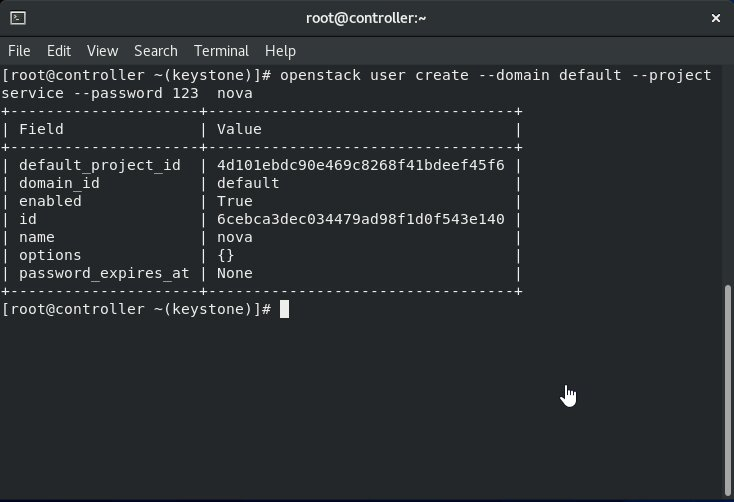
\includegraphics[width=1\linewidth]{Cloud/Nova Setup in Keystone/Create [Nova] User In [Service] Project} 
\end{center} 
\caption{Create [Nova] User In [Service] Project} 
\end{figure}  \FloatBarrier 
\\
\begin{figure}[!htb] 
\begin{center} 
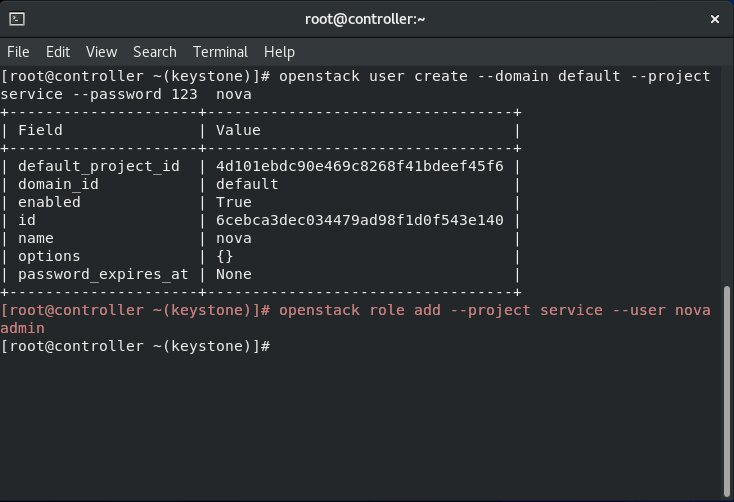
\includegraphics[width=1\linewidth]{Cloud/Nova Setup in Keystone/Add [Nova] User In [Admin] Role} 
\end{center} 
\caption{Add [Nova] User In [Admin] Role} 
\end{figure}  \FloatBarrier 
\\

\section{Installing Keystone}

\par Next, we will assign this new user the role of administrator. Likewise, we
let's create a user of type placement and also give him the role of administrator. 
\\
\begin{figure}[!htb] 
\begin{center} 
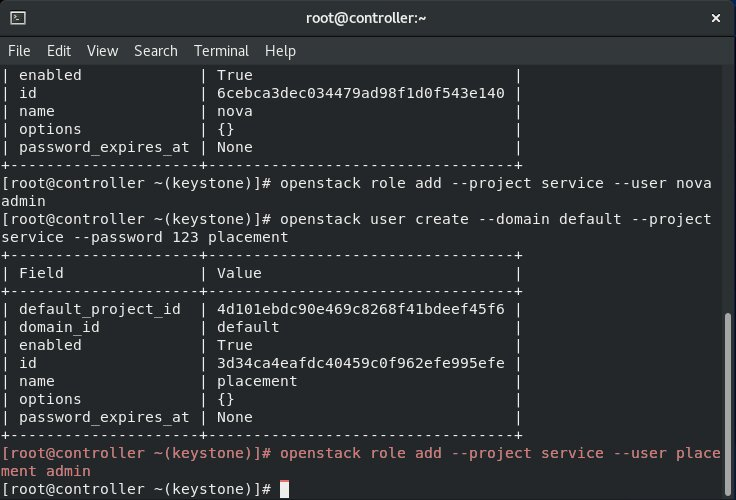
\includegraphics[width=1\linewidth]{Cloud/Nova Setup in Keystone/Add [Placement] User In [Admin] Role}
\end{center} 
\caption{Add [Placement] User In [Admin] Role} 
\end{figure}  \FloatBarrier 
\\
\par Now we are going to create a service entry for nova and another for placement. 
\begin{figure}[!htb] 
\begin{center} 
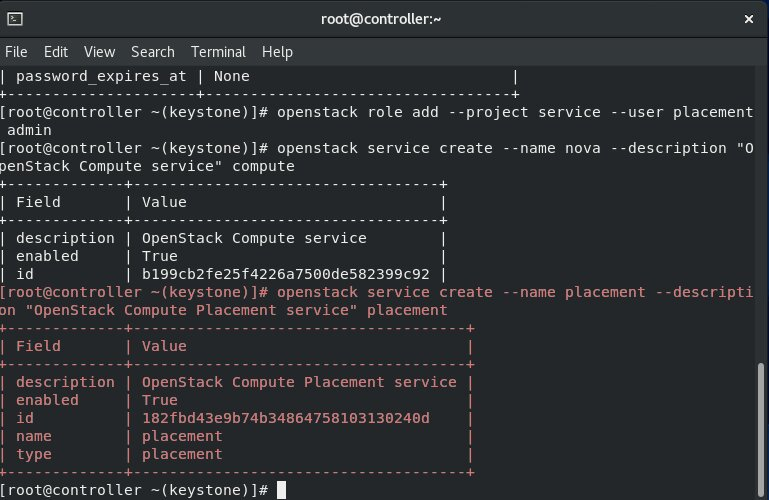
\includegraphics[width=1\linewidth]{Cloud/Nova Setup in Keystone/Create Service Entry For [Placement]} 
\end{center} 
\caption{Create Service Entry For [Placement]} 
\end{figure}  \FloatBarrier 
\\

\par We must define the nova API as host and create an endpoint for nova and placement in interfaces
public, internal and admin  .\\

\\
\begin{figure}[!htb] 
\begin{center} 
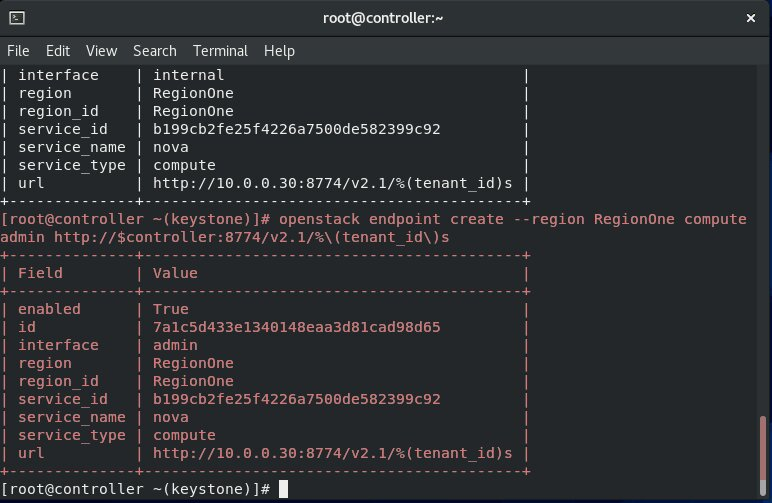
\includegraphics[width=1\linewidth]{Cloud/Nova Setup in Keystone/Create Endpoint For [Nova] (Admin)} 
\end{center} 
\caption{Create Endpoint For [Nova] (Admin)} 
\end{figure}  \FloatBarrier 
\\
\\
\begin{figure}[!htb] 
\begin{center} 
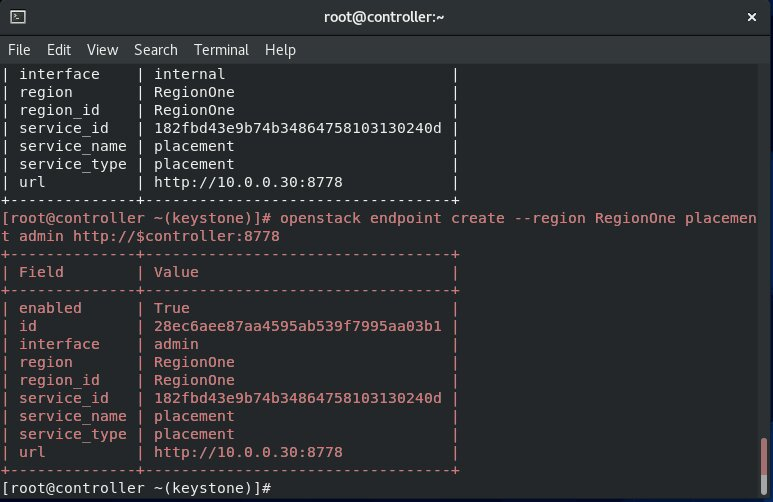
\includegraphics[width=1\linewidth]{Cloud/Nova Setup in Keystone/Create Endpoint For [Placement] (Admin)} 
\end{center} 
\caption{Create Endpoint For [Placement] (Admin)} 
\end{figure}  \FloatBarrier 
\\
\subsection{Adding a Database on MariaDB for Nova}
\par We will then add the nova, placement, nova api and nova cell0 databases to our Mariadb. 
\\
\begin{figure}[!htb] 
\begin{center} 
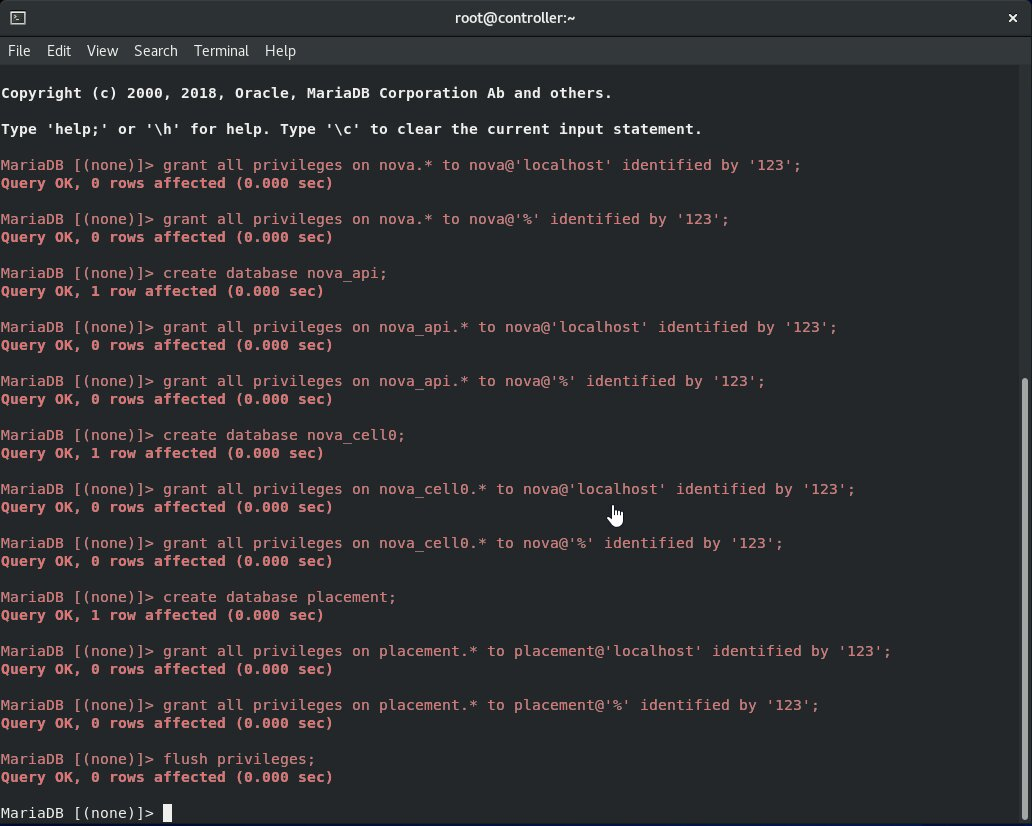
\includegraphics[width=1\linewidth]{Cloud/Nova Setup in Keystone/Add A User And Database On Mariadb For Nova} 
\end{center} 
\caption{Add A User And Database On Mariadb For Nova} 
\end{figure}  \FloatBarrier 
\\

\section{Installing and Configuring Nova services}
\subsection{Installing Nova services}
\par 
Now it's time to install Nova services and then configure it. 
\\
\begin{figure}[!htb] 
\begin{center} 
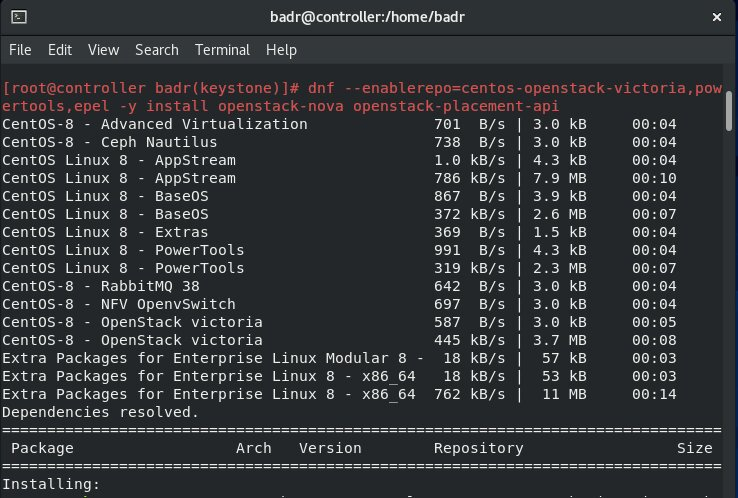
\includegraphics[width=1\linewidth]{Cloud/Installing and Configuring Nova services/Installing Nova services} 
\end{center} 
\caption{Installing Nova services} 
\end{figure}  \FloatBarrier 
\\

\subsection{Configuring Nova}
\par 
For the configuration, we will rename the file etc/nova/nova.conf.org in
Etc/nova/nova.conf.\newline Here is the contents of the file: 
\\
\begin{figure}[!htb] 
\begin{center} 
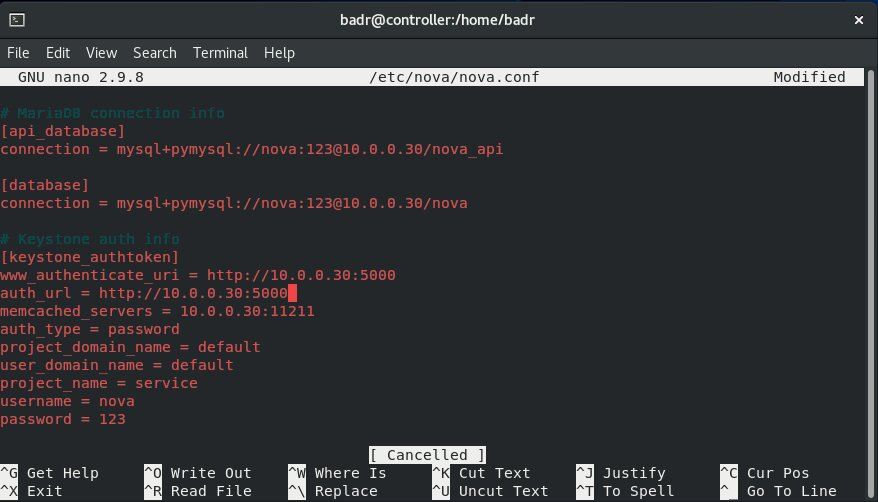
\includegraphics[width=1\linewidth]{Cloud/Installing and Configuring Nova services/Creating nova.conf} 
\end{center} 
\caption{Creating nova.conf} 
\end{figure}  \FloatBarrier 
\\

\par 
We are going to change the access permissions to this file with the chmod 640 command which means
that the owner has read and write rights, that the group has read-only rights and that
all other users have no rights to the file.
\\
\begin{figure}[!htb] 
\begin{center} 
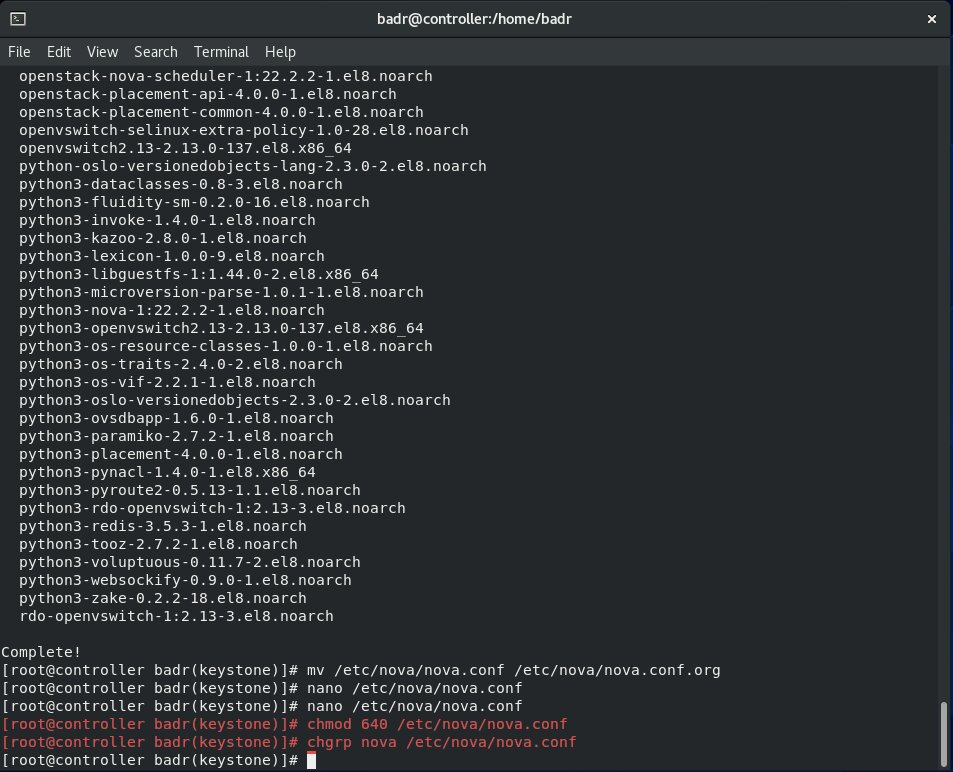
\includegraphics[width=1\linewidth]{Cloud/Installing and Configuring Nova services/nova.conf access} 
\end{center} 
\caption{nova.conf access} 
\end{figure}  \FloatBarrier 
\\


\par now we do the same thing for the placement.conf file
\\
\begin{figure}[!htb] 
\begin{center} 
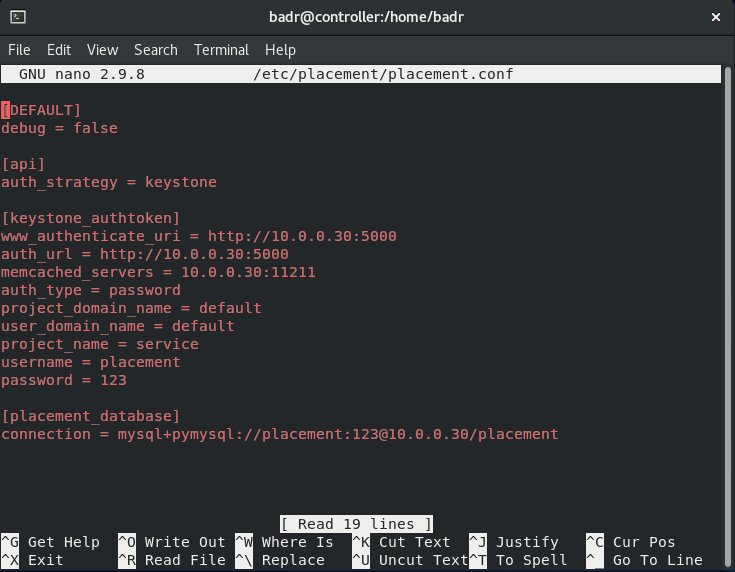
\includegraphics[width=1\linewidth]{Cloud/Installing and Configuring Nova services/Creating placement.conf} 
\end{center} 
\caption{Creating placement.conf} 
\end{figure}  \FloatBarrier 

\\
\begin{figure}[!htb] 
\begin{center} 
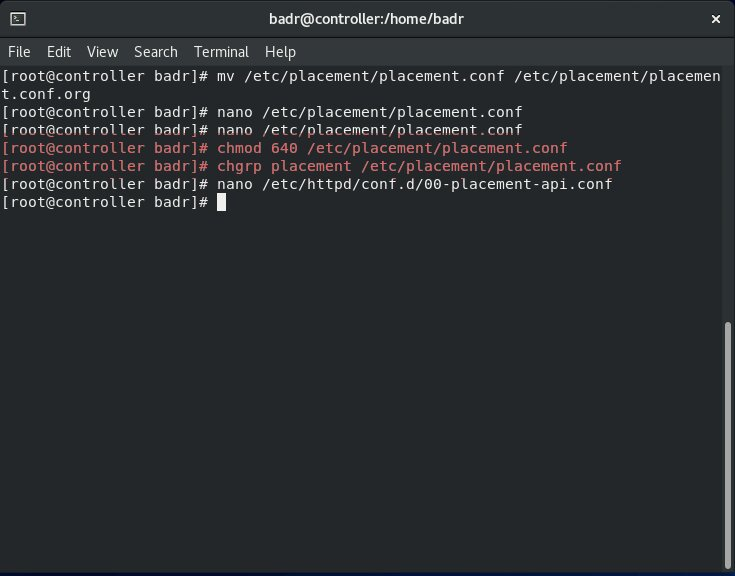
\includegraphics[width=1\linewidth]{Cloud/Installing and Configuring Nova services/placement.conf access} 
\end{center} 
\caption{placement.conf access} 
\end{figure}  \FloatBarrier 
\\
\\
\begin{figure}[!htb] 
\begin{center} 
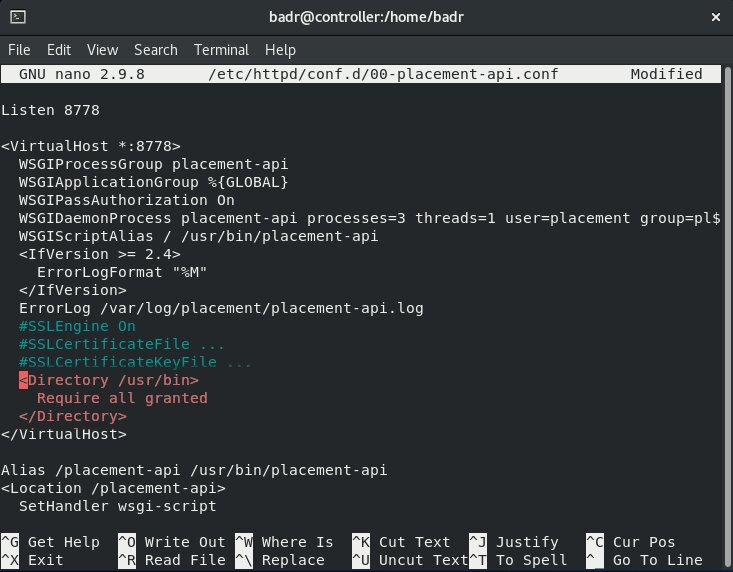
\includegraphics[width=1\linewidth]{Cloud/Installing and Configuring Nova services/Changing 00-placement-api.conf} 
\end{center} 
\caption{Changing 00-placement-api.conf} 
\end{figure}  \FloatBarrier 
\\
\subsection{novaapi.te config}
\par We will install openstack-selinux using dnf and we will adjust the port to be
tcp 8778. Here is the content of the novaapi.te file 
\\
\subsection{Starting Nova services}
\par We will then chain these commands to change the SELinux policy: 
\\

\begin{figure}[!htb] 
\begin{center} 
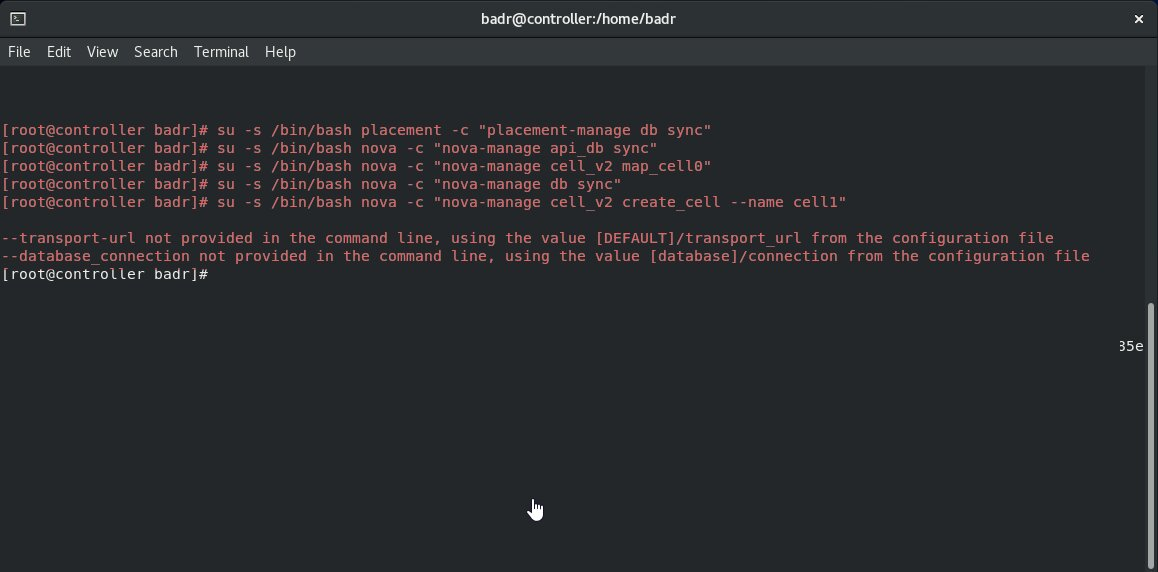
\includegraphics[width=1\linewidth]{Cloud/Installing and Configuring Nova services/Add Data into Database} 
\end{center} 
\caption{Add Data into Database} 
\end{figure}  \FloatBarrier 
\\
\par The status of nova-conductor and nova-scheduler are UP: 
\\
\begin{figure}[!htb] 
\begin{center} 
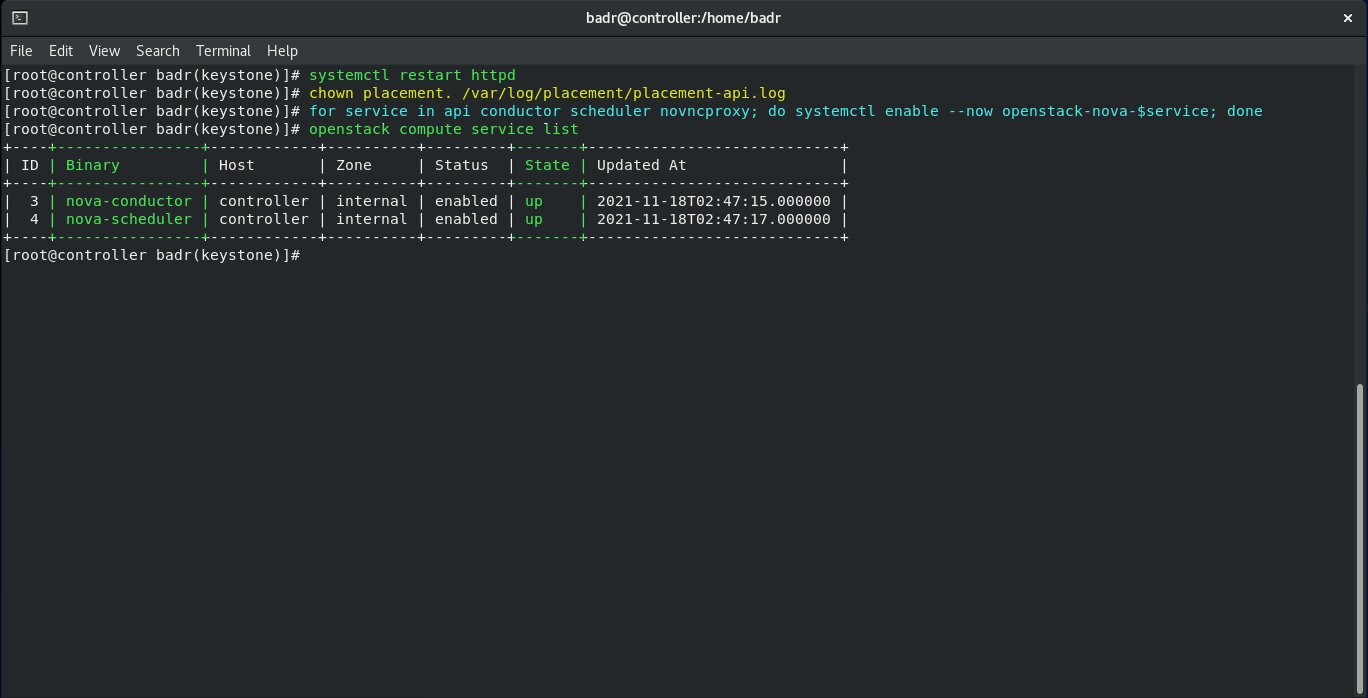
\includegraphics[width=1\linewidth]{Cloud/Installing and Configuring Nova services/Show Compute status} 
\end{center} 
\caption{Show Compute status} 
\end{figure}  \FloatBarrier 
\\
\section{Installing and Configuring Nova Compute}
\subsection{Installing Nova Compute}
\par After installing the KVM hypervisor we will install nova compute.

\\
\begin{figure}[!htb] 
\begin{center} 
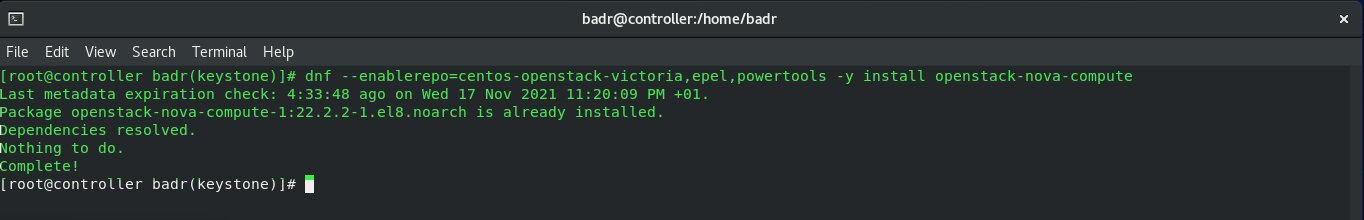
\includegraphics[width=1\linewidth]{Cloud/Installing and Configuring Nova Compute/Install Nova Compute} 
\end{center} 
\caption{Install Nova Compute} 
\end{figure} 
\FloatBarrier
\\
\subsection{nova.conf config}
\par In addition to basic settings of Nova, we will add the following settings to the nova.conf file in order to enable VNC.
\\
\begin{figure}[!htb] 
\begin{center} 
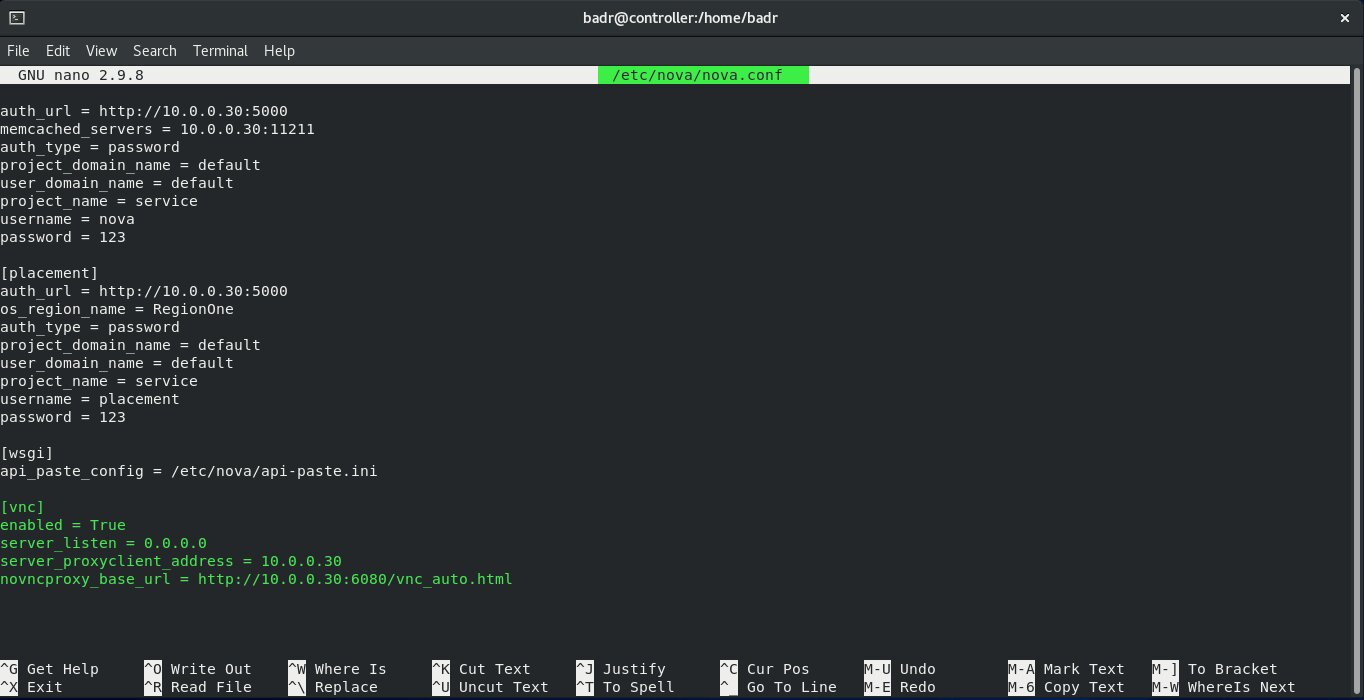
\includegraphics[width=1\linewidth]{Cloud/Installing and Configuring Nova Compute/Add Follows (Enable Vnc)} 
\end{center} 
\caption{Add Follows (Enable Vnc)} 
\end{figure} 
\FloatBarrier
\\

\subsection{Start Nova Compute}

\par First thing is changing the SELinux policy and enabling openstack-nova-compute,and finally starting the Nova Compute 
\\
\begin{figure}[!htb] 
\begin{center} 
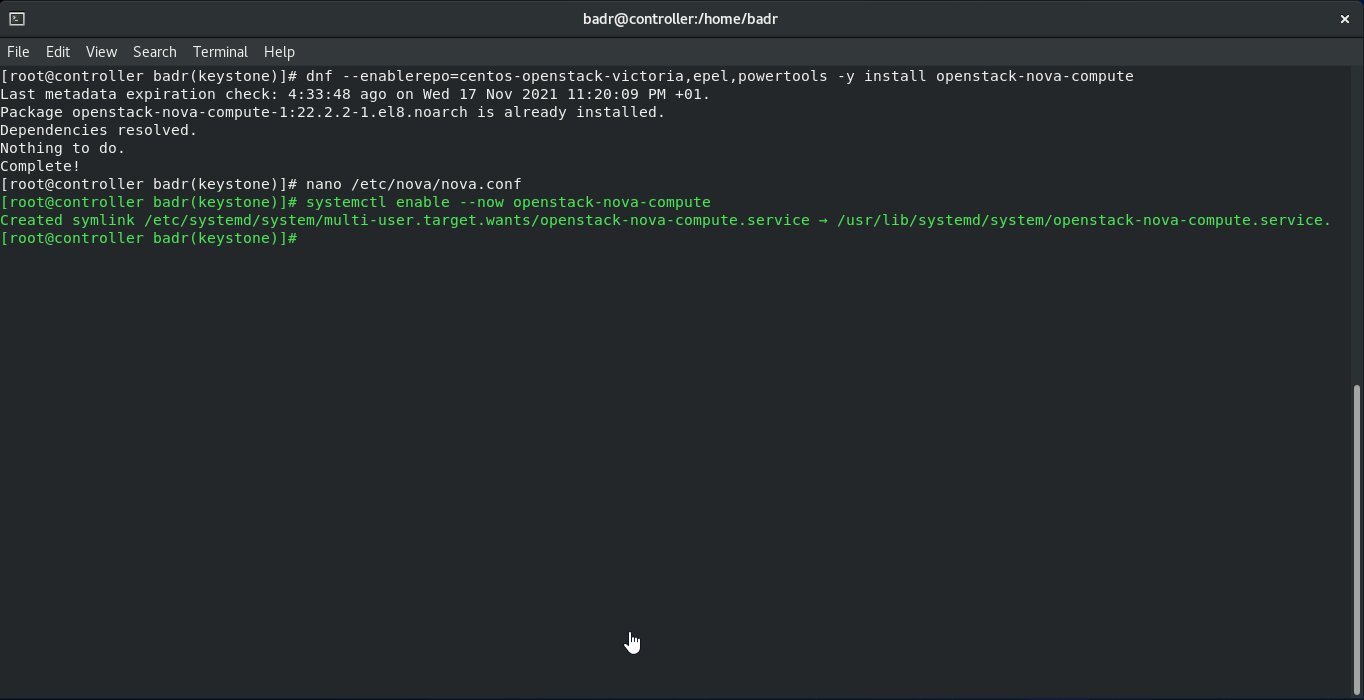
\includegraphics[width=1\linewidth]{Cloud/Installing and Configuring Nova Compute/Start Nova Compute} 
\end{center} 
\caption{Start Nova Compute} 
\end{figure} 
\FloatBarrier
\\
\\
\begin{figure}[!htb] 
\begin{center} 
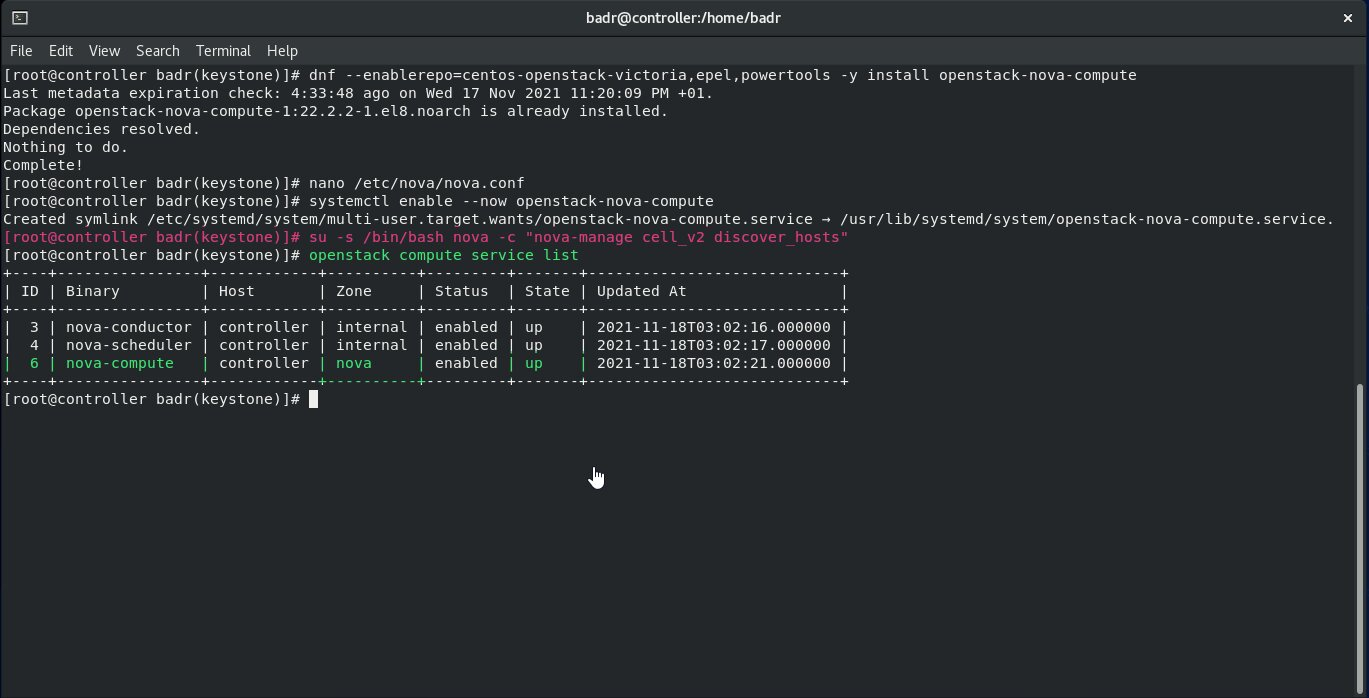
\includegraphics[width=1\linewidth]{Cloud/Installing and Configuring Nova Compute/Show Status} 
\end{center} 
\caption{Show Status} 
\end{figure} 
\FloatBarrier
\\



\end{spacing}